\documentclass[UTF8,12pt]{article} % 12pt 为字号大小
\usepackage{amssymb,amsfonts,amsmath,amsthm}
\usepackage{times}
\usepackage{graphicx} % 插图
\usepackage{cite}
\usepackage{xeCJK}
\usepackage{color}
\usepackage{caption}
\usepackage{placeins} % 防止浮动
%----------
% 插入代码的格式定义
% 参考 https://www.latexstudio.net/archives/5900.html
%----------
\usepackage{listings}
\lstset{
 columns=fixed,       
 numbers=left,                                        % 在左侧显示行号
 numberstyle=\tiny\color{gray},                       % 设定行号格式
 frame=none,                                          % 不显示背景边框
 backgroundcolor=\color[RGB]{245,245,244},            % 设定背景颜色
 keywordstyle=\color[RGB]{40,40,255},                 % 设定关键字颜色
 numberstyle=\footnotesize\color{darkgray},           
 commentstyle=\it\color[RGB]{0,96,96},                % 设置代码注释的格式
 stringstyle=\rmfamily\slshape\color[RGB]{128,0,0},   % 设置字符串格式
 showstringspaces=false,                              % 不显示字符串中的空格
 language=c++,                                        % 设置语言
}
%----------
% 算法伪代码
% https://blog.csdn.net/lwb102063/article/details/53046265
%----------
\usepackage{algorithm}  
\usepackage{algpseudocode}  
\usepackage{amsmath}  
\renewcommand{\algorithmicrequire}{\textbf{Input:}}  % Use Input in the format of Algorithm  
\renewcommand{\algorithmicensure}{\textbf{Output:}} % Use Output in the format of Algorithm  



%----------
% 字体定义
%----------


\newcommand*{\songti}{\CJKfamily{zhsong}} % 宋体
\newcommand*{\heiti}{\CJKfamily{zhhei}}   % 黑体
\newcommand*{\kaiti}{\CJKfamily{zhkai}}  % 楷体
\newcommand*{\fangsong}{\CJKfamily{zhfs}} % 仿宋
\newcommand*{\lishu}{\CJKfamily{zhli}}    % 隶书
\newcommand*{\yuanti}{\CJKfamily{zhyou}} % 圆体

%----------
% 版面设置
%----------
%首段缩进
\usepackage{indentfirst}
\setlength{\parindent}{2em}
%行距
\renewcommand{\baselinestretch}{1.25} % 1.25倍行距
%页边距
\usepackage[a4paper]{geometry}
\geometry{verbose,
  tmargin=2cm,% 上边距
  bmargin=2cm,% 下边距
  lmargin=2cm,% 左边距
  rmargin=2cm % 右边距
}

% ----------
% 多级标题格式在此设置
% https://zhuanlan.zhihu.com/p/32712209
% \titleformat{command}[shape]%定义标题类型和标题样式,字体
% {format}%定义标题格式:字号(大小),加粗,斜体
% {label}%定义标题的标签,即标题的标号等
% {sep}%定义标题和标号之间的水平距离
% {before-code}%定义标题前的内容
% [after-code]%定义标题后的内容
% ----------
\usepackage{titlesec} %自定义多级标题格式的宏包
% 三级标题
% 4
\titleformat{\section}[block]{\large \bfseries}{\arabic{section}}{1em}{}[]
% 4.1
\titleformat{\subsection}[block]{\normalsize \bfseries}{\arabic{section}.\arabic{subsection}}{1em}{}[]
% 4.1.1
\titleformat{\subsubsection}[block]{\small \mdseries}{\arabic{section}.\arabic{subsection}.\arabic{subsubsection}}{1em}{}[]
\titleformat{\paragraph}[block]{\footnotesize \bfseries}{[\arabic{paragraph}]}{1em}{}[]


%----------
% 其他宏包
%----------
%图形相关
\usepackage[x11names]{xcolor} % must before tikz, x11names defines RoyalBlue3
\usepackage{graphicx}
\usepackage{pstricks,pst-plot,pst-eps}
\usepackage{subfig}
\def\pgfsysdriver{pgfsys-dvipdfmx.def} % put before tikz
\usepackage{tikz}

%原文照排
\usepackage{verbatim}

%链接的格式
\usepackage[colorlinks,linkcolor=red]{hyperref}
%表格
\usepackage{tabularx}

%==========
% 正文部分
%==========
\captionsetup[figure]{labelsep=period}
\captionsetup[table]{labelsep=period}

\begin{document}
\renewcommand{\figurename}{图}
\renewcommand{\tablename}{表}
\renewcommand{\refname}{参考文献}

% \kaiti 是楷体,参见上面的字体设置
\title{\bf{\heiti 计算机前沿技术成果复现计划}}
\author{\normalsize{姓名: XX}\hspace{2cm}\normalsize{学号: XX}}
\date{}
\maketitle



\section{拟复现原文}

\textbf{Example: NDC: Neural Dual Contouring (SIGGRAPH 2022)}

\textbf{\textcolor[rgb]{1,0,0}{(请说明是否已开源。如已有源码,请详细说明你复现的不同点,将增加何种操作或功能来提升原文的性能表现)}}


\subsection{论文主要内容概述}

该论文利用XXXXX

\begin{figure}[ht]
  \centering
  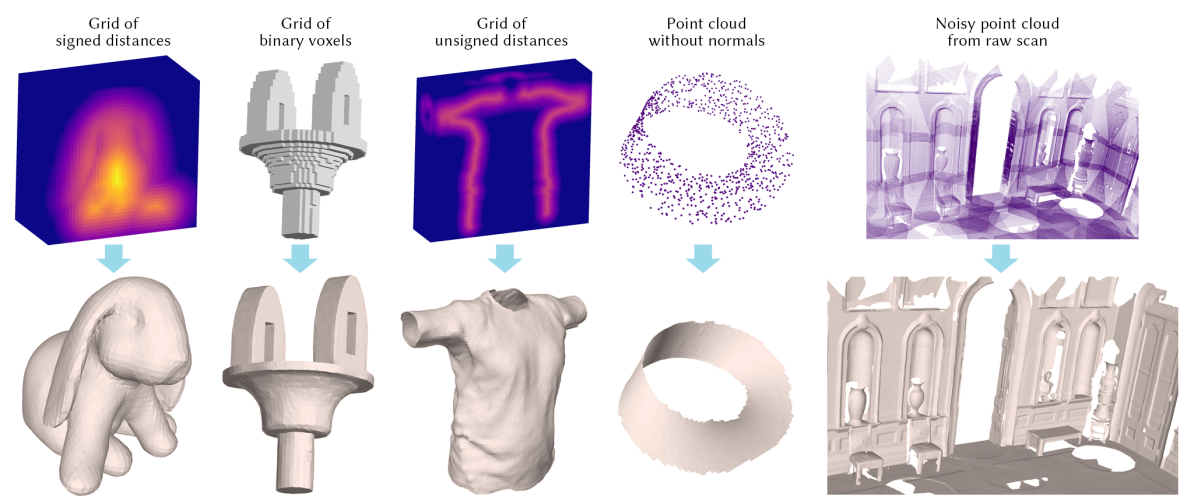
\includegraphics[scale=0.4]{figs/fig1.png}
  \captionsetup{font={scriptsize,stretch=1}}
  \caption{NDC是一种采用数据驱动方式学习从各种输入重建网格,包括带符号或无符号距离场、体素、点云和嘈杂的原始扫描。经过 CAD 模型训练,NDC 可以推广到各种形状类型,包括具有锐利边缘的 CAD 模型、布料的开放表面、室内场景,甚至是不可定向的莫比乌斯带。}
  \label{fig:enc-dec}
\end{figure}

\subsection{论文主要技术创新点}

\begin{itemize}
    \item XXXX
    \item XXXX
\end{itemize}



\section{复现工作说明}

\subsection{选择理由}

XXX

\subsection{拟复现的具体内容}

\begin{itemize}
    \item XXXX
    \item XXXX
\end{itemize}

\subsection{预期结果和演示}

XXXX


\section{复现工作计划进度}

XXXXX


\begin{table}[H]
    \centering
    \begin{tabular}{c|c}
    \hline
    \textbf{时间安排}         & \textbf{预计进度} \\ \hline
    202X年XX月XX日 - 202X年XX月XX日 & 论文阅读整理        \\
    XXX                   & XXX           \\
    XXX                   & XXX           \\ \hline
    \end{tabular}
    \captionsetup{font={small,stretch=1}}
    \caption{预期复现计划进度安排}
    \label{tab:my_schedule}
\end{table}



\bibliography{refs}
\bibliographystyle{plain}




\end{document}